\section{system overview}
\label{sec:system}

\begin{figure}[th]
\centering
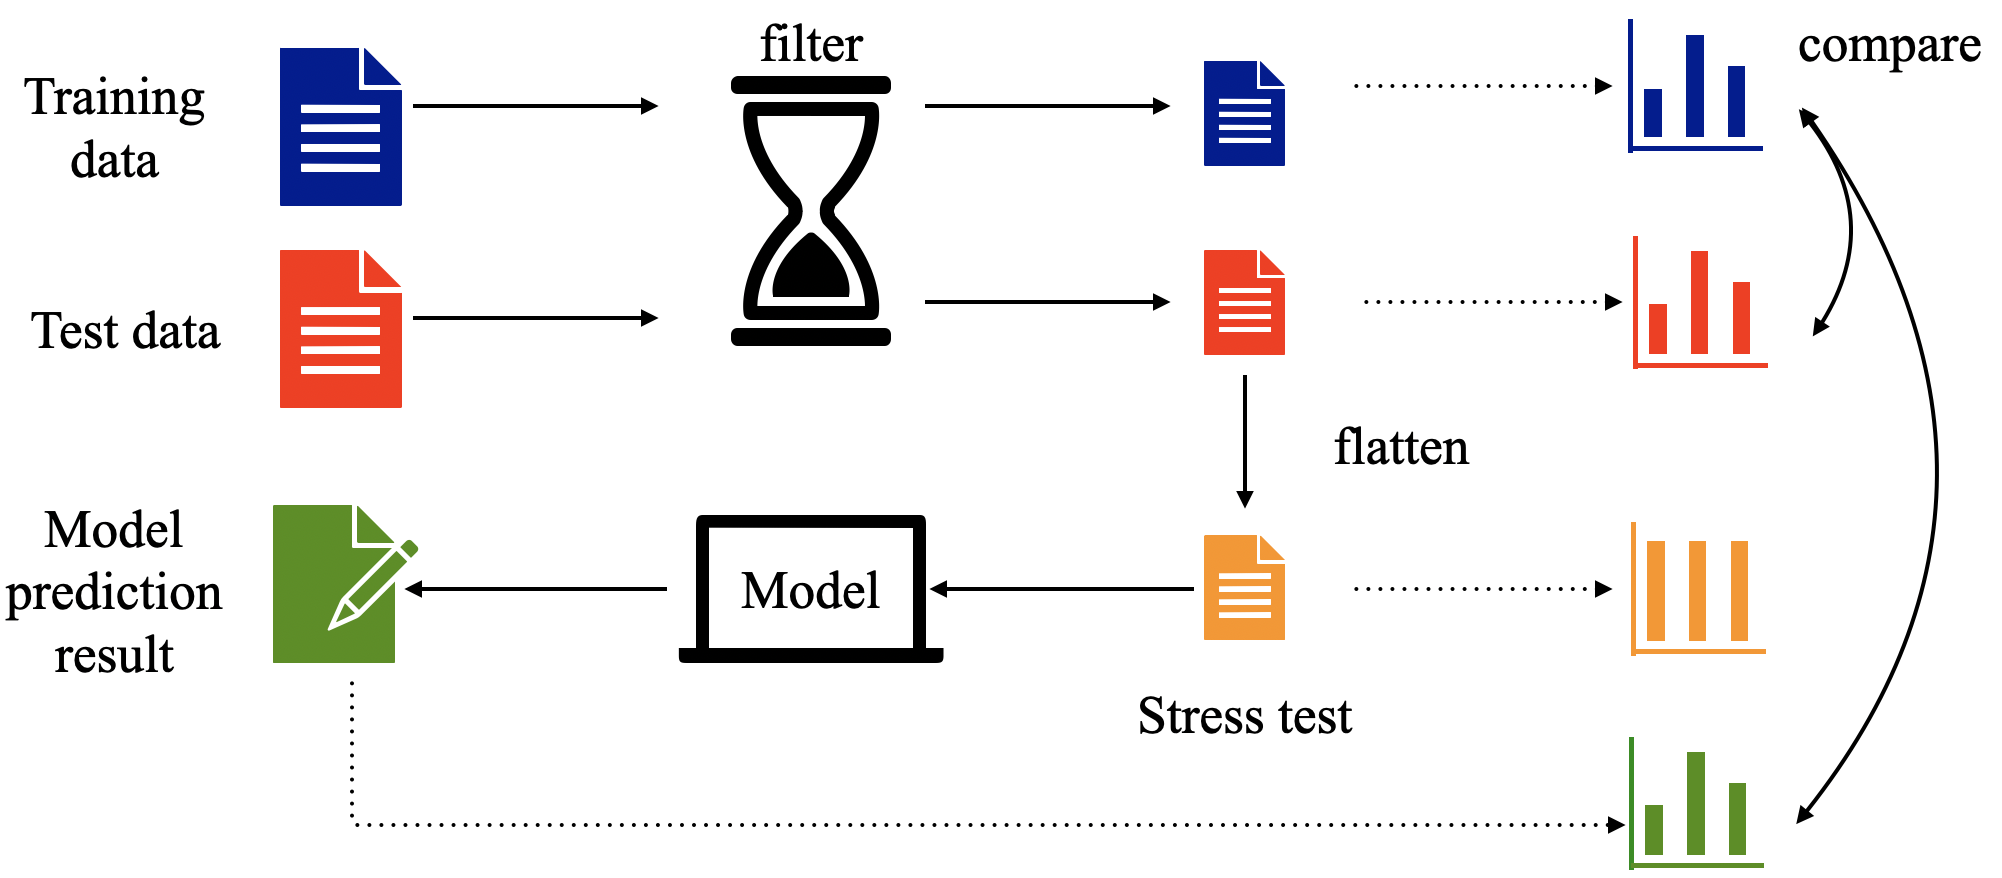
\includegraphics[width=1.0\columnwidth]{picture/framework.jpg}
\caption{Workflow}
\label{fig:framework}
\end{figure}

As illustrated in~\figref{fig:framework}, at the phase of data analysis, 
cue samples extraction, cue test data generation 
and distribution comparison, we can get to know 
whether the data have cue problem and analysis what features a model is really sensitive 
to in reasoning tasks.

%WeWe evaluate the information leak in the datasets by statistical cues only. 
%First, we formulate  a number of NL reasoning tasks in a general form. 
%Then based on the cues associated with each label, 
%we design a number of metrics to measure the correlation between words
%and labels. Such correlation scores are called ``cue scores'' because they are 
%indicative of potential cue patterns. Afterwards, we aggregate the scores using a number of simple statistical
%models to make the predictions. Finally, we show how to split a dataset into
%the easy and hard parts using the above fast predictions.

\subsection{Task Formulation}

%\textcolor{red}{Hongru: these are concrete examples, which i think should be given after the problem
%formulation} 
Given question instance $x$ of a natural language reasoning (NLR) task dataset $X$ 
we mentioned above, we formulate it as
\begin{equation}
    x = (p, h, l) \in X,
\end{equation}
\noindent
where $p$ is the context against which to do the reasoning, and $p$ corresponds 
to ``premise'' in~\exref{exp:snli};
$h$ is the hypothesis given the context $p$. $l \in \mathcal{L}$ is the label that 
depicts the type of relation between $p$ and $h$. 
The size of the relation set $\mathcal{L}$ varies between tasks. We argue that 
most of the discriminative NLR tasks can be formulated into this general form. 
%which will bring us much convenience to evaluate the cues of a dataset. 
For example, an NLI question consists of a \textit{premise}, a \textit{hypothesis} 
and a \textit{label} on the relation between premise and hypothesis. 
%The formulation of this task will be $p =$ \textit{premise}, $q =$ \textit{hypothesis} and $l =$ \textit{label}. 
$|\mathcal{L}| = 3$ for three different relations: 
\textit{entailment}, \textit{contradiction} and \textit{neutral}. 
We will talk about how to transform into this form in \secref{sec:dynamic}. 
%The ROCStory~\cite{mostafazadeh2016corpus} dataset
%such as in~\exref{exp:roc}, 
%consists of a \textbf{context} and two possible story \textbf{endings}. 

%We will formulate this task by setting $p = $ \textit{context}, $h = $ \textit{ending1/ending2}. In this case, $|\mathcal{L}| = 2$. because $l$ is ``true'' or ``false'' indicating whether 
%the ending is a plausible ending of the story.
\subsection{Analysis Data}


We need to analysis train dataset, test dataset and model prediction.

\subsection{Extract Samples Based on Features}
\label{sec:extract}

We suggest that users consider at least the following features: Word (unigram word in the task), 
Typos, NER (appropriately understanding named entities), 
Tense(understanding order of events), Negation, 
Sentiment, Overlap(overlap words between premise and hypothesis). 
This listing of cues is not exhaustive, but a starting point for users, 
who should also come up with additional features that are specific 
to their task or domain. We use $F$ to denote feature set.

\subsubsection{Word} For a dataset $X$, 
we collect a set of all words $\mathcal{N}$ that exist in $X$. 
%These 
%words can be word or cross-word that consists of a pair of
%unigrams, one from the premise and other from the hypothesis.
%the token pair between $p$ and $h$.
The feature metric for a word measures the disparity of the word's appearance under 
 a specific label. 
%The cross-unigrams, such as  ``swimmer-sea'' in~\exref{exp:snli}, 
%represent the 
%relational unigrams in a dataset. 
%The ``swimmer-sea'' cross-unigram can be identified as a cue if it always appear in the instances with 
%one label, like entailment.

Let $w$ be a word in $\mathcal{N}$, we compute a scalar statistic metric 
called {\em cue score}, $f^l$,  we use conditional probability(CP)
as the feature score to measure the correlation between words and labels 

\begin{equation}
    f^{(w,l)} = \frac{\#(w, l)}{\#(w)}
\end{equation}

We rank the words by feature score to $N^{'}$ and 
only treat top $k$ words as features:

\begin{equation}
    F_{W_i} = {w}_{i} , i \in 1...k \wedge w_{i} \in N^{'}
\end{equation}.
%of $w$ with respect to label $l$ as
%%\KZ{Consider changing $\mathcal{F}$ to $\mathcal{B}$ to avoid confusion with $f$?}
%
%\begin{equation}
%    f_{\mathcal{F}}^{l} = f_{\mathcal{F}}(w, l),    
%\end{equation}
%%We call $f_{\mathcal{F}}^{(k,l)}$ \textit{cue metric}, 
%where $f_{\mathcal{F}}^{l}$ is a function which measures how much spurious information can be conveyed by token $w_k$ for a particular label $l$. 
%$\mathcal{F}$ is a set of cue metrics that we used for computing the \textit{cue score}. 

\subsubsection{Sentiment}

We assigned sentiment features $F_{S}$as 
positive, negative, or neutral sentiment to each hypothesis which 
represented as: 
$S(h) = sign(number of positive words - number of negative words) in the hypothesis$.
The sentiment polarity of a word
is determined by a look-up from pre-trained
sentiment lexica\footnote{nltk}. 

\subsubsection{Tense}

Considering the order of events can is also an 
important information for commonsense reasoning, we include 
\textit{past}, \textit{present}, \textit{future} as Tense features $F_{Tense}$. 
The tense is determined by verb tags of dependency parsing~\footnote{scipy}.

\subsubsection{Negation}

Many work has observed that 
strong negation words (“no”, “not”) cause the model to predict contradiction for
neutral or entailed statements .Thus we think negation feature $F_{Neg}$can be a factor which affect models 
to make decisions. Negation is also decided on dependency parsing tags.

\subsubsection{Overlap}

In many cases, large word-overlap between premise and hypothesis sentences causes
wrong entailment prediction, even if they are unrelated. 
Very little word overlap causes a prediction
of neutral instead of entailment. Thus we wonder to 
know whether overlap feature $F_{O}$ can 
really influence models.

\subsubsection{NER}

The failure for the NER tests in CheckList~\cite{}
indicates that these models are relying on shortcuts
such as anchoring on named entities too strongly
instead of understanding named entities and their
impact on whether questions are duplicates. We also 
take in NER feature $F_{NER}$ in our feature test.

\subsubsection{Typos}

The premise or the hypothesis is ill-formed because of spelling errors. 
Typo feature $F_{Typos}$ many also can be learned by models as off-site information. 
We use a pretrained spelling model to get the typo information in a 
sentence. 

Given the features $F$, we can extract samples which contain a specific 
feature for training dataset and test dataset. In~\figref{fig:framework}, the blue 
distribution and red distribution represent  train and test data distribution based on 
a certain feature. We use mean square deviation(MSD) to measure the balance rate 
of a feature in a dataset. Then, we can observe which feature of the test set 
is insufficient for testing if the filtered test data size is quite small or samples on 
some label is rare which bellow a threshold $\sigma$. 
We can point out what kind of test samples should be augmented. 
but don't provide new method for data augmentation. 
%We only pay attention to the features which have enough test data for model evaluation.
%In addition, we can analysis the credibility of test data through 
%the Kullback-Leibler (KL) Divergence. If a train dataset distribution is unbalance, 
%a similar distribution between train and T
%test can lead to insufficient test which test the cues mostly with a certain label. 


\subsection{Generate stress test data}
\label{sec:generate}

We require a more fair dataset to test if a model is sensitive to a feature.
The extracted test dataset in \figref{fig:framework} (red) is unbalance with 
labels. Thus We assign a threshold for the smallest in test samples 
organized by different labels to decide whether this feature can be well tested 
with filtered dataset. If the test samples are adequate, we even-out the samples 
with various labels just as the yellow part in \figref{fig:framework}. Then we test the model 
on the reconstructed feature test data, the similarity between prediction result (green) and 
training data distribution(blue) on a feature indicates how the model is influenced by 
the appearance of the feature in training data. The similarity is 
calculated by Kullback-Leibler (KL) Divergence.

\subsection{Transformation of MCQs with dynamic choices}
\label{sec:dynamic}
So far the multiple-choice questions we targeted such as NLI problems
are actually classification problems with fixed set of choices. There is
another type of language reasoning tasks which are also in the form of
multiple-choice questions, but their choices are not fixed, as shown
below. 
\begin{example}\label{exp:roc}
An example question in ROCStory~\cite{mostafazadeh2016corpus}.\\
\noindent
\textbf{Context}: Rick grew up in a troubled household. 
He never found good support in family, and turned to gangs.           
It was n't long before Rick got shot in a robbery.             
The incident caused him to turn a new leaf.\\
\noindent
\textbf{Ending 1}: He joined a gang. \\
\noindent
\textbf{Ending 2}:  He is happy now.\\
\noindent
\textbf{Answer}: 2
\end{example}

In this type of tasks,
we can separate the original story into two unified instances, 
$u_1=(context, ending1, false)$ and $u_2=(context, ending2, true)$.
We can predict the label with probability for each instance $\mathcal{G}(input(u_1);\phi)$ and 
 $\mathcal{G}(input(u_2);\phi)$.
Then we can choose the ending with higher probability to make the prediction.
%For better take advantage of the bias score to choose the right choice. We also use two linear model: SGDClassifier and 
%logistic regression. The inputs of the models for instance $e_n$ is the concatenation of bias scores for each label which %can express as :  $input(e_n) = [ f_{\mathcal{F}}^{(w_{n_1}^{l_1})},..., f_{\mathcal{F}}^{(w_{n_d}^{l_1})},..., f_{\mathcal{F}}^{(w_{n_1}^{l_v})},..., f_{\mathcal{F}}^{(w_{n_d}^{l_v})}]$. The corresponding target is the correct label $l_{gold}\in{L}$.

 

